\chapter{評価}
\begin{large}
\begin{quote}
本章では,本システムの評価を行う.
\end{quote}
\end{large}
\clearpage

\section{評価方針}
本節では,本システムが
\ref{sec:requirements}で示した機能要件を満たしているかどうかを
実験を行うことで評価する.
具体的な方法について以下に述べる.


\begin{enumerate}
\item{リアルタイム性}\\
本研究は環境モニタリングやターゲットトラッキングのような
無線センサネットワークにおけるアプリケーションを対象としているため,
イベントモデルである拡張する前のContikiと本システムの比較し,
リアルタイムタスク発生から実行までの時間を評価する.
\newline
\item{省資源性かつ低オーバヘッド}\\
本システムではリアルタイム処理が必要なイベントが発生しない場合には,
イベントモデルを採用している.
本要件が満たされているかどうかを確認するために,
純粋なスレッドモデルであるNano-RK上で同様の動作をするアプリケーションを実行し,
その際に消費される電力について評価を行う.
\end{enumerate}




%一般的なイベント駆動型のオペレーティングシステムでは,
%タスクは実行待ち状態になった順に実行されるため,
%重要なタスクが実行されず,
%そのタスク実行時にはその価値がなくなってしまうこともあるだろう.
%リアルタイム処理をサポートすれば,
%重要なタスクから順に処理を実行していくため,
%このように重要なタスクを未処理のまま終えてしまうような
%事態を未然に防ぐことができる.
%
%リアルタイム処理をサポートすることにより,
%低消費電力での運用も実現可能となる.
%リアルタイムタスクを効率的に処理可能なオペレーティングシステムと,
%効率の悪いオペレーティングシステムを比較した場合,
%前者の方が同じ精度のサービスを実現する場合に
%低いクロックで動作することができる.
%また,センサノード上では無線やセンサなどの
%周辺デバイスは必要のないときにスリープされることで消費電力を抑えている.
%このとき,リアルタイムタスクが処理可能ならば,
%素早く周辺デバイスのオンとオフを
%切り替えることができるようになるため,
%低消費電力を維持することが期待される.
%さらに,リアルタイム処理をサポートすることで,
%効率的に無線資源を利用し,
%無線通信に伴う電力を削減することができるだろう.

\section{評価環境}


\begin{table}[htb]
  \centering
  \caption{実験結果1}
  \begin{tabular}{|c||c|c|c|c|c|} \hline
    \backslashbox{}{} & 最小値 & 最大値 & 中央値 & 平均値 & 標準偏差 \\ \hline \hline
    D-Switch & 80 & 82 & 81 & 81 & 0.17 \\ \hline
    Contiki & 80 & 163 & 81 & 97.97 & 33.39 \\ \hline
  \end{tabular}
  \label{tab:latency1}
\end{table}

\begin{figure}[htbp]
 \begin{center}
  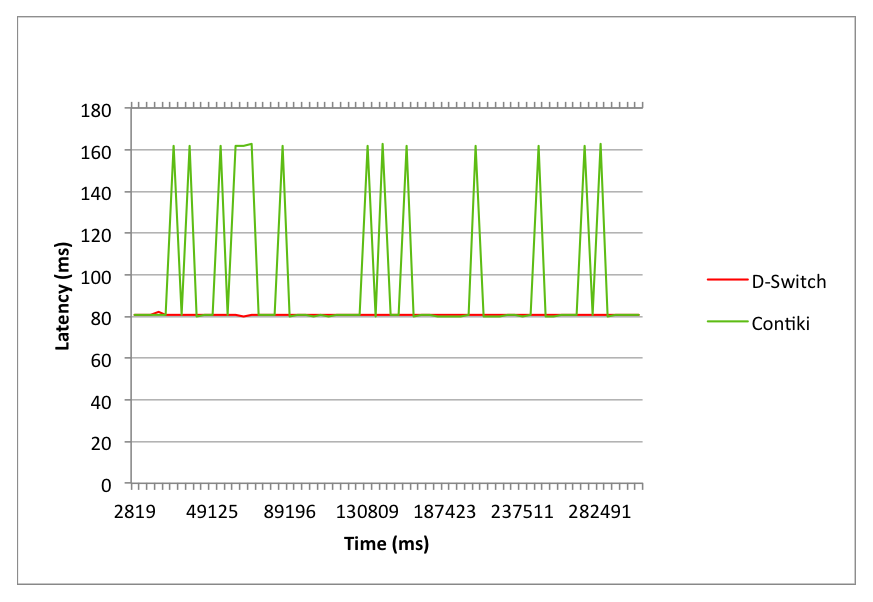
\includegraphics[width=120mm]{./images/latency1.eps}
 \end{center}
 \caption{実験結果1}
 \label{fig:latency1}
\end{figure}

\begin{figure}[htbp]
 \begin{center}
  \includegraphics[width=120mm]{./images/cdf1.eps}
 \end{center}
 \caption{実験結果1}
 \label{fig:cdf1}
\end{figure}


\begin{table}[htb]
  \centering
  \caption{実験結果2}
  \begin{tabular}{|c||c|c|c|c|c|} \hline
    \backslashbox{}{} & 最小値 & 最大値 & 中央値 & 平均値 & 標準偏差 \\ \hline \hline
    D-Switch & 80 & 82 & 81 & 81.02 & 0.19 \\ \hline
    Contiki & 80 & 163 & 81 & 108.37 & 38.49 \\ \hline
  \end{tabular}
  \label{tab:latency2}
\end{table}

\begin{figure}[htbp]
 \begin{center}
  \includegraphics[width=120mm]{./images/latency2.eps}
 \end{center}
 \caption{実験結果2}
 \label{fig:latency2}
\end{figure}

\begin{figure}[htbp]
 \begin{center}
  \includegraphics[width=120mm]{./images/cdf2.eps}
 \end{center}
 \caption{実験結果2}
 \label{fig:cdf2}
\end{figure}


\begin{table}[htb]
  \centering
  \caption{実験結果3}
  \begin{tabular}{|c||c|c|c|c|c|} \hline
    \backslashbox{}{} & 最小値 & 最大値 & 中央値 & 平均値 & 標準偏差 \\ \hline \hline
    D-Switch & 81 & 82 & 81 & 81.02 & 0.24 \\ \hline
    Contiki & 80 & 245 & 81 & 98.36 & 49.61 \\ \hline
  \end{tabular}
  \label{tab:latency3}
\end{table}

\begin{figure}[htbp]
 \begin{center}
  \includegraphics[width=120mm]{./images/latency3.eps}
 \end{center}
 \caption{実験結果3}
 \label{fig:latency3}
\end{figure}

\begin{figure}[htbp]
 \begin{center}
  \includegraphics[width=120mm]{./images/cdf3.eps}
 \end{center}
 \caption{実験結果3}
 \label{fig:cdf3}
\end{figure}





\begin{table}[htb]
  \centering
  \caption{実験結果4}
  \begin{tabular}{|c||c|c|c|c|c|} \hline
    \backslashbox{}{} & 最小値 & 最大値 & 中央値 & 平均値 & 標準偏差 \\ \hline \hline
    D-Switch & 81 & 81 & 81 & 81 & 0 \\ \hline
    Contiki & 80 & 326 & 81 & 102 & 48.52 \\ \hline
  \end{tabular}
  \label{tab:latency4}
\end{table}

\begin{figure}[htbp]
 \begin{center}
  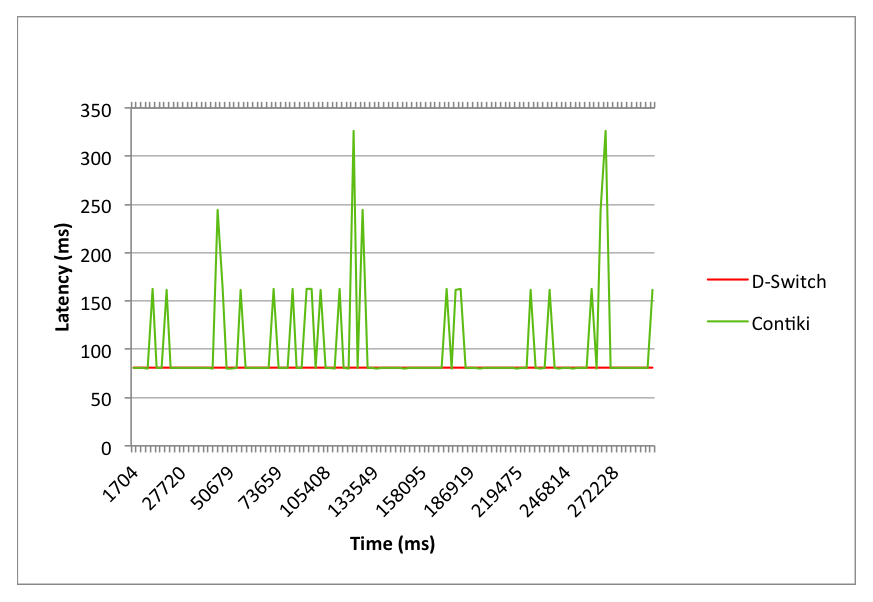
\includegraphics[width=120mm]{./images/latency4.eps}
 \end{center}
 \caption{実験結果4}
 \label{fig:latency4}
\end{figure}

\begin{figure}[htbp]
 \begin{center}
  \includegraphics[width=120mm]{./images/cdf4.eps}
 \end{center}
 \caption{実験結果4}
 \label{fig:cdf4}
\end{figure}



\begin{table}[htb]
  \centering
  \caption{実験結果5}
  \begin{tabular}{|c||c|c|c|c|c|} \hline
    \backslashbox{}{} & 最小値 & 最大値 & 中央値 & 平均値 & 標準偏差 \\ \hline \hline
    D-Switch & 80 & 82 & 81 & 81.02 & 0.21 \\ \hline
    Contiki & 80 & 327 & 81 & 121.26 & 63.95 \\ \hline
  \end{tabular}
  \label{tab:latency5}
\end{table}

\begin{figure}[htbp]
 \begin{center}
  \includegraphics[width=120mm]{./images/latency5.eps}
 \end{center}
 \caption{実験結果5}
 \label{fig:latency5}
\end{figure}

\begin{figure}[htbp]
 \begin{center}
  \includegraphics[width=120mm]{./images/cdf5.eps}
 \end{center}
 \caption{実験結果5}
 \label{fig:cdf5}
\end{figure}




\section{考察}

\section{まとめ}
%本章では,まず,本研究に評価方針,実験環境を述べた.次に,実験環境内における実験への影響を調査するため,それぞれのリージョンからICMPにおける,Message Requestを送信し,リプライが返されるまでの時間(RTT)を計測した.その結果,RTTは0.400ms以内であり,十分に無視できることを述べた.次いで,保存ピア探索における計算コスト,データの保存に要する時間,データの取得に要する時間の観点から評価を行った.その結果から,考察を行い,理論値と実際の値に齟齬が存在することを明らかにし,その違いは,T-Ringにおいて,保存や取得の対象となるデータの時間情報の取得を行う際に要する時間により生じていることに言及した.
